\chapter{Aplicação de validação da API proposta} \label{cap:aplicacao_exemplo}

  Para validar a API construída, o protocolo de comunicação proposto entre a API e o módulo Matemático
  e a arquitetura proposta em geral, foram criados a aplicação cliente do Pentano e um módulo matemático
  que implementa o algoritmo k-Means para a clusterização.
  Todas as aplicações construídas, inclusive a API proposta, se encontram no repositório do Pentano\footnote{\href{https://gitlab.com/pentano}{https://gitlab.com/pentano}}.
  
  \begin{figure}[h!]
    \centering
    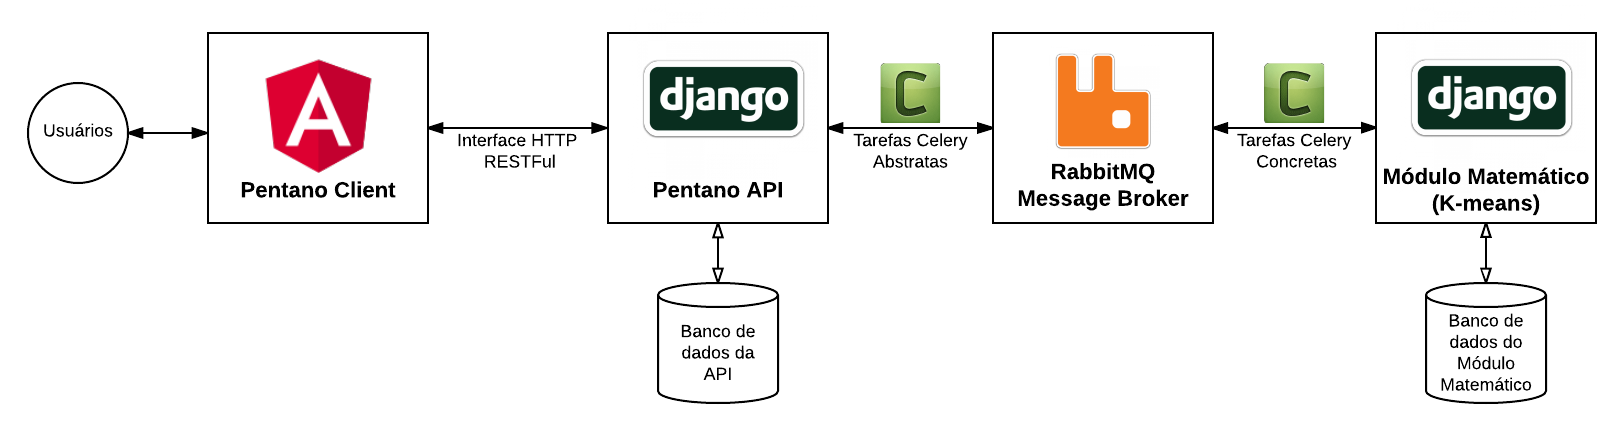
\includegraphics[scale=0.4]{figuras/whole_solution.png}
    \caption{Solução completa utilizando a arquitetura proposta.}
    \label{fig:whole_solution}
  \end{figure}
  
  A Figura \ref{fig:whole_solution} apresenta a solução completa implementada, que
  é composta por:
  
  \begin{enumerate}
      \item a aplicação cliente do Pentano, que é uma aplicação \textit{web} amigável ao usuário que fornece 
      fácil acesso aos serviços providos pela API;
      \item a API do Pentano, que fornece os serviços de autenticação e gerenciamento das conversas, comentários e votos; 
      \item uma instância do módulo matemático,
	  que fornece o serviço de clusterização para agrupar os usuários; e
      \item uma instância do RabbitMQ\footnote{\href{https://www.rabbitmq.com/}{https://www.rabbitmq.com/}} para
	  intermediar a comunicação entre a API e o módulo matemático, servindo como meio de transporte das
	  mensagens disparadas pelo Celery.
	  
  \end{enumerate}

  Nas próximas seções são apresentados os detalhes de cada parte desta solução implementada
  para validar a arquitetura proposta.
  
%     Colocar links para os repos
  
  \section{Aplicação Cliente e API}
    
    A aplicação cliente é a interface gráfica para os serviços de 
    gerenciamento de conversas, comentários e votos providos pela API e foi
    criada para consolidar as funcionalidades desenvolvidas e fornecer uma interface mais
    amigável para o sistema. Foram implementados todos os requisitos descritos na seção \ref{functional_requirements}
    em uma aplicação Angular 2\footnote{\href{https://angular.io/}{https://angular.io/}} para
    testar a integração com todos os \textit{endpoints} da API e demonstrar o comportamento da API. Esta aplicação foi feita utilizando os recursos providos pelo próprio \textit{framework}, portanto
    possui uma arquitetura baseada em componentes, claramente apresentada na própria documentação do Angular.
    
    
    Resumidamente, a arquitetura consiste em uma hierarquia de componentes organizados
    em módulos independentes que se comunicam para compor a aplicação e realizar o objetivo desejado.
    Cada componente conta com um \textit{template} HTML e uma classe para gerenciar o comportamento do componente.
    Cada módulo pode possuir serviços, que são classes que encapsulam a lógica da aplicação.
    É a partir da camada de serviços que a integração com a API é realizada.
    
    Quando um nova conversa, comentário ou voto são criados na aplicação cliente,
    a API é invocada para a criação do respectivo dado, que por sua vez
    notitifica o módulo matemático da ação recém ocorrida para que o mesmo possa reagir de acordo.
    Essa comunicação é feita através de tarefas do Celery e são transportadas como mensagens assíncronas
    através do RabbitMQ para o módulo matemático.
    
    A Figura \ref{fig:cliente} apresenta uma das telas da aplicação criada. 
    Nessa tela é representada uma conversa criada a título de exemplificação
    com seus comentários e os grupos de usuários formados. Cada cor representa um grupo e cada círculo representa um usuário. 
    
    \begin{figure}[h!]
      \centering
      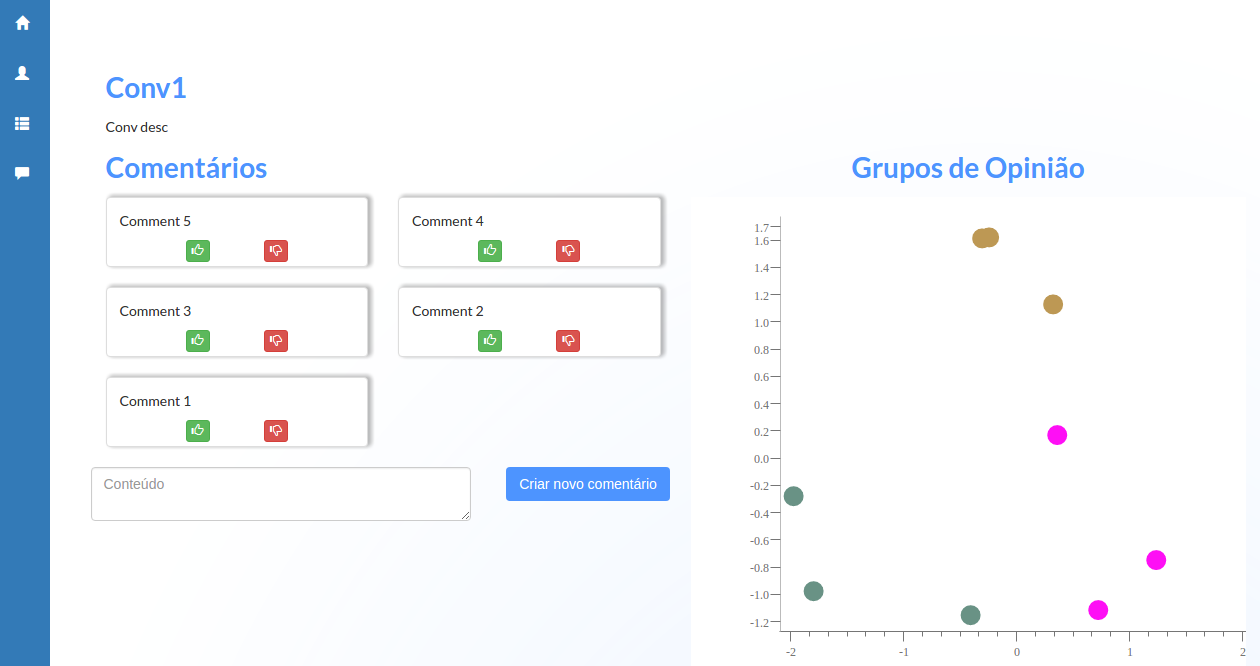
\includegraphics[scale=0.48]{figuras/client.png}
      \caption{Tela que apresenta os comentários e grupos de usuáŕios de uma conversa}
      \label{fig:cliente}
    \end{figure}
  
    Nesta implementação, ao serem criados conversas, comentários e votos, o módulo matemático
    sincroniza seu banco de dados com os novos dados.
     
  \section{Módulo matemático}
     
    Quando a aplicação cliente solicita os dados dos grupos de usuários de uma conversa,
    a API delega ao módulo matemático responder o dado solicitado. A partir daí o módulo
    matemático começa a trabalhar, realizando todo o processo de clusterização dos usuários
    a partir dos votos em comentários da respectiva conversa solicitada.
    
    Em um trabalho anterior \cite{tallys_tcc}, o módulo matemático foi criado utilizando o algoritmo k-Means, descrito no Capítulo \ref{cap:classificação},
    para realizar a composição dos \textit{clusters} de usuários. No escopo deste trabalho esse módulo foi adaptado e refatorado para contemplar
    o protocolo de comunicação estabelecido.
    As implementações realizadas foram feitas utilizando recursos matemáticos
    providos pela bibloteca Python \textit{scikit-learn}\footnotemark 
    e os detalhes da implementação de \citeonline{tallys_tcc} são apresentados a seguir.
    \footnotetext{http://scikit-learn.org/stable/}
    
    
    A cada solicitação dos \textit{clusters} de uma conversa
    o fluxo apresentado na Figura \ref{fig:resumo_clusterizao_ej} é realizado.
    Para cada conversa, os $P$ votos realizados nos $N$ comentários são a entrada para o módulo de clusterização, 
    gerando uma entrada de dimensão $N$. 
    
    
    \begin{figure}[h!]
      \centering
      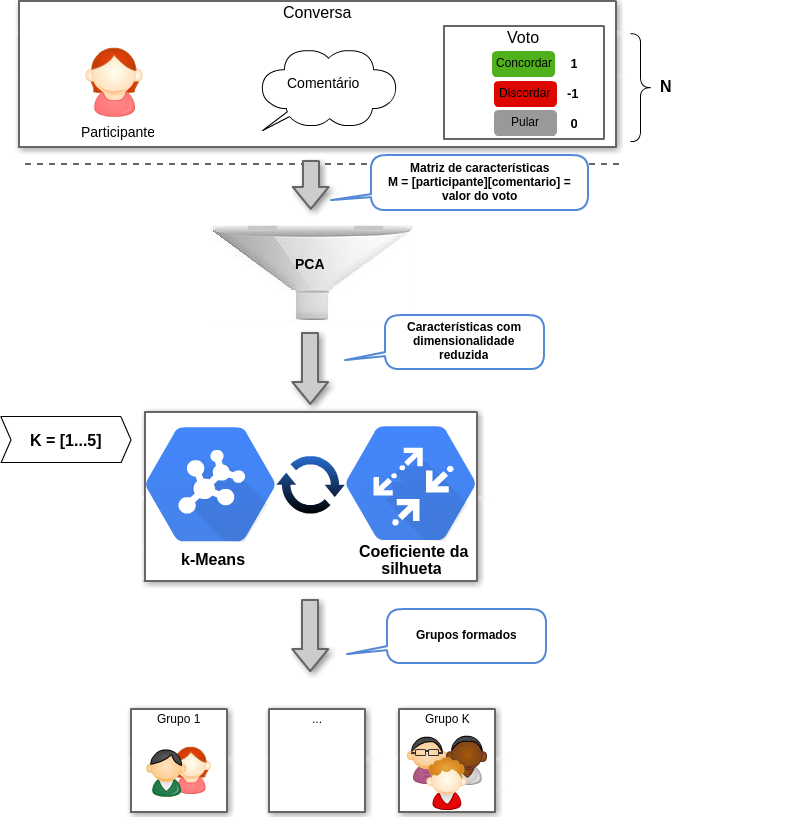
\includegraphics[scale=0.6]{figuras/resumo_clusterizao_ej.png}
      \caption{Fluxo de clusterização do ``Empurrando Juntos''}
      \label{fig:resumo_clusterizao_ej}
    \end{figure}
  

    Frequentemente antes de medir a similaridade entre os objetos é necessário
    reduzir a dimensionalidade, isso acontece, pois para espaços de alta dimensão as distâncias euclidianas
    tendem a inflar. Reduzir a dimensionalidade pode aliviar esse problema e diminuir o tempo de cálculo.
    Um dos métodos mais utilizados para realizar essa redução é a Análise de 
    Componentes Principais (PCA, do inglês) \cite{han2011data, sklearn}.

    \citeonline{mackiewicz1993principal} afirmam que a redução de dimensionalidade no PCA é
    obtida com a criação de uma nova combinação linear das variáveis que caracterizam os
    objetos estudados, satisfazendo condições matemáticas e estatísticas.
    \citeonline{shlens2014tutorial} afirma que o principal objetivo da técnica é identificar
    uma base para expressar um conjunto de dados que elimine os ruídos e revele 
    outros dados escondidos. Isso acontece com a criação de $n$ vetores ortogonais que possuem o mesmo significado que o conjunto
    de vetores inicial, porém em um conjunto menor \cite{han2011data}. 
    
    Considerando isso, é aplicada a técnica de PCA para que
    a dimensionalidade da combinação de comentário e votos seja reduzida. 
    Com os dados em duas dimensões, para possibilitar a visualização gráfica, 
    é aplicado o algoritmo k-Means, para obtenção da disposição dos grupos de pessoas. 
    
    Para a definição do melhor valor para $k$, foi aplicada uma técnica analítica conhecida como Coeficiente de Silhueta \cite{tan2013data}.  
    Essa técnica tem por objetivo combinar a avaliação de coesão e separação dos \textit{clusters} por meio do cálculo de um coeficiente (o de silhueta) que 
    varia de -1 a 1, no qual um coeficiente negativo representa que o elemento está no \textit{cluster} errado.
    O valor ``zero'' representa que o elemento está próximo da ``borda'' do \textit{cluster} e por fim, quanto mais próximo do valor 1, melhor
    está a distribuição dos \textit{clusters}.

    Dessa forma, com a escolha de um intervalo de valores para $k$, como sugerido por \citeonline{han2011data} e \citeonline{sklearn}, é possível testar os valores 
    para o coeficiente de silhueta e escolher o melhor valor de $k$ dentro do intervalo. 

    No fluxo de clusterização do ``Empurrando Juntos'', o k-Means é aplicado em ciclos para a descoberta do melhor valor de 
    $k$ por meio do cálculo do coeficiente de silhueta.
    No final dos ciclos, na saída do fluxo são formados os grupos de pessoas com opiniões semelhantes, que são retornados para API.
 
    Os dois módulos apresentados neste capítulo complementaram a arquitetura definida para o ``Empurrando Juntos'',
    do ponto de vista funcional, e permitiram a visualização do funcionamento da API e do sistema por completo.
    
    \section{Resultados e Discussão}
    
    A aplicação de validação proposta neste Capítulo trata-se de uma validação relacionada ao comportamento de resposta
    dos protocolos de comunicação estabelecidos, os \textit{endpoints}
    e o protocolo definido. Nesse sentido, a arquitetura de comunicação definida mostrou-se adequada 
    para a proposta do trabalho, na qual o módulo matemático deve ser configurado no momento da implantação do sistema completo, 
    ou seja, os três módulos. 
    
    As tecnologias de troca de mensagens para o protocolo de comunicação, Celery e RabbitMQ, funcionaram 
    apropriadamente nos testes com a configuração
    da comunicação apenas de uma aplicação para outra. 
    
    As funcionalidades de deleção já estavam previstas na API, contudo não estavam previstas tarefas na interface
    de comunicação para sincronizar os módulos matemáticos. Após a construção da aplicação, foi percebida a necessidade de acrescentar
    as duas tarefas de deleção no protocolo.
    
    
    
    
      
      